\documentclass[sigconf]{webmedia}

\usepackage{lmodern}
%webmeda.cls is adapted from acmart.cls for use in Proceedings of the Brazilian Symposium on Multimedia and the Web (WebMedia)

%% Pacotes adicionais deste trabalho (não alteram margens, fontes ou espaçamentos)
\usepackage[brazil]{babel}
\graphicspath{{figuras/}{./}}  % aceita as figuras em figuras/ ou na raiz

%%
%% \BibTeX command to typeset the BibTeX logo in the docs
\AtBeginDocument{%
  \providecommand\BibTeX{{%
    \normalfont B\kern-0.5em{\scshape i\kern-0.25em b}\kern-0.8em\TeX}}}

\settopmatter{printacmref=false, printfolios=false}

%% Evento: trabalho acadêmico da disciplina (mesma classe/estilo do WebMedia)
\setevent{webmedia}
\proceedingsDetails[Teoria dos Grafos 2026]{Trabalho Prático de Teoria dos Grafos -- Instituto de Computação, UFBA}{2026}{Salvador/BA, Brasil}
%\ISSN{2966-2753}

\begin{document}

\title[Analisando o grafo email-EuAll do SNAP]{Análise Estrutural e Algorítmica do Grafo \texttt{email-EuAll} do SNAP}
\subtitle{Trabalho Prático -- Analisando Grafos do SNAP (G34)}

\author{Igor Reis Santos}
\email{igorreis@ufba.br}
\affiliation{%
  \institution{Instituto de Computação, Universidade Federal da Bahia}
  \city{Salvador}
  \state{Bahia}
  \country{Brasil}
}

\renewcommand{\shortauthors}{Igor Reis Santos}

\begin{abstract}
Este trabalho analisa o grafo \texttt{email-EuAll} do SNAP, uma rede de e-mails de uma
instituição de pesquisa europeia com 265.214 vértices e 420.045 arestas dirigidas,
atribuído pela regra de mapeamento da matrícula (G34). Após remover auto-loops,
converter o grafo para não dirigido simples e extrair a maior componente conexa
(224.832 vértices e 339.925 arestas), calculamos as propriedades estruturais clássicas,
obtendo diâmetro (14) e raio (7) exatos por meio do algoritmo \emph{BoundingDiameters}.
Implementamos e medimos o tempo de BFS, DFS, verificação de Eulerianidade, Dijkstra,
Bellman-Ford, Floyd-Warshall, Tarjan, Prim e Kruskal, reportando média, desvio padrão e
intervalo de confiança de 95\%. A rede é fortemente \emph{small-world}
($\sigma \approx 2{,}7\times10^{4}$), tem distribuição de graus de cauda pesada,
compatível apenas aproximadamente com uma lei de potência, e é robusta a falhas
aleatórias, mas colapsa quando os 5\% de vértices mais centrais, por grau ou por
PageRank, são removidos.
\end{abstract}

\keywords{teoria dos grafos, redes complexas, SNAP, email-EuAll, small-world, lei de potência, robustez}

\maketitle

%% ===================================================================
\section{Introdução}

Grafos permitem estudar sistemas reais (redes sociais, de comunicação, de
infraestrutura) por meio de propriedades estruturais que não aparecem em análises
tabulares. Este trabalho aplica os conceitos da disciplina a um grafo real do
repositório SNAP~\cite{snapnets}, cobrindo três frentes: (i) a análise estrutural
obrigatória (Parte~I); (ii) a implementação dos algoritmos estudados, com análise de
complexidade teórica e observada (Parte~II); e (iii) a investigação das propriedades
\emph{small-world}, lei de potência e robustez (Parte~III).

Todos os algoritmos e análises foram implementados pelo autor em Python. A biblioteca
NetworkX~\cite{hagberg2008} foi usada apenas para validar os resultados nos testes
automatizados e para desenhar a visualização. O texto está organizado da seguinte forma:
a Seção~\ref{sec:calculo} apresenta o cálculo do grafo; a Seção~\ref{sec:codigo}, o
repositório; as Seções~\ref{sec:grafo} e~\ref{sec:tratamento}, o grafo e o tratamento;
a Seção~\ref{sec:metodologia}, a metodologia; a Seção~\ref{sec:resultados}, os
resultados; e as Seções~\ref{sec:discussao} e~\ref{sec:conclusao}, a discussão crítica
e a conclusão.

%% ===================================================================
\section{Determinação do Grafo}
\label{sec:calculo}

Dado o número de matrícula $M$, seja $S$ a soma dos seus dígitos e $U$ o número formado
pelos seus dois últimos dígitos. O índice do grafo é
\begin{equation}
  G = \big(S \times (U + 1)\big) \bmod 129,
\end{equation}
usando-se $G = 129$ caso o resultado seja zero. Para a matrícula $M = 224216275$:
\begin{align*}
  S &= 2+2+4+2+1+6+2+7+5 = 31, \qquad U = 75,\\
  G &= (31 \times 76) \bmod 129 = 2356 \bmod 129 = 2356 - 18\times129 = 34.
\end{align*}
O grafo G34 da planilha \textsc{Analisando-SNAP-Dataset} é o \texttt{email-EuAll}
(categoria \emph{Communication networks}).

%% ===================================================================
\section{Código e Dados}
\label{sec:codigo}

O código-fonte, o conjunto de dados tratado, as tabelas e figuras geradas e o
\texttt{README} com as instruções de execução estão disponíveis em
\url{https://github.com/igor377/grafos-snap-email-euall}. O pipeline completo é executado
por \texttt{python scripts/run\_all.py}, e o notebook \texttt{notebooks/analise.ipynb}
reúne todos os resultados. As implementações são conferidas contra o NetworkX por
110 testes automatizados (\texttt{python -m pytest}).

%% ===================================================================
\section{Descrição do Grafo Original}
\label{sec:grafo}

O \texttt{email-EuAll}~\cite{leskovec2007,snapnets} foi construído a partir dos e-mails
de uma grande instituição de pesquisa europeia trocados entre outubro de 2003 e março de
2005. Cada vértice é um endereço de e-mail, e há uma aresta dirigida $u \rightarrow v$ se
$u$ enviou ao menos um e-mail para $v$. Segundo a documentação do SNAP, o grafo de
comunicação é completo apenas para os 1.258 endereços da própria instituição. Apenas
34.203 endereços enviaram \emph{e} receberam mensagens no período, e os demais são
endereços externos, inexistentes, digitados incorretamente ou de spam. O arquivo é distribuído
como lista de arestas (\texttt{.txt.gz}), com 265.214 vértices (identificadores
$0,\dots,265.213$, sem lacunas) e 420.045 arestas dirigidas. O grafo é \textbf{não
ponderado} e não traz o instante de cada mensagem: as arestas já vêm agregadas no
período.

%% ===================================================================
\section{Tratamento dos Dados}
\label{sec:tratamento}

Os tratamentos foram aplicados na ordem abaixo, e a Tabela~\ref{tab:tratamento} mostra
o efeito de cada etapa.

\begin{enumerate}
  \item \textbf{Remoção de auto-loops:} 1.089 arestas $u \rightarrow u$ foram removidas.
  Elas não afetam caminhos e distorceriam graus e testes de Eulerianidade.
  \item \textbf{Dirigido $\rightarrow$ não dirigido simples:} as arestas $u\rightarrow v$
  e $v\rightarrow u$ viram uma única aresta $\{u,v\}$. As métricas da Parte~I, os
  caminhos mínimos, as árvores geradoras e a robustez são definidos sobre a relação
  ``houve comunicação'', que é simétrica.
  \item \textbf{Extração da maior componente conexa (LCC):} diâmetro, raio e comprimento
  médio só são finitos em grafos conexos. A LCC preserva 84,8\% dos vértices e 93,3\% das
  arestas, e é também a política adotada para grafo desconexo no Apêndice~C (robustez).
  \item \textbf{Grafo dirigido preservado:} a versão dirigida sem auto-loops foi mantida
  para o algoritmo de Tarjan, pois na versão não dirigida cada componente conexa seria
  trivialmente uma única componente fortemente conexa.
  \item \textbf{Redução por custo computacional:} um subgrafo induzido de 300 vértices,
  obtido por BFS a partir de um vértice aleatório da LCC (372 arestas, conexo), é usado
  em Bellman-Ford e Floyd-Warshall.
\end{enumerate}

Não houve tratamento temporal nem de multigrafo, porque o arquivo não contém
\emph{timestamps} nem arestas repetidas. Como o grafo é não ponderado, os algoritmos
ponderados usam \textbf{pesos sintéticos} inteiros uniformes em $[1,10]$, sorteados com
semente fixa (42). O subgrafo herda os pesos da LCC.

% Gerado por src/report_tables.py a partir de results/tables/ -- não editar
\begin{table}[t]
  \caption{Evolução do grafo ao longo do tratamento.}
  \label{tab:tratamento}
\small
\begin{tabular}{lrr}
  \toprule
  Etapa & Vértices & Arestas \\
  \midrule
  Grafo bruto (dirigido) & 265.214 & 420.045 \\
  Sem auto-loops (dirigido) & 265.214 & 418.956 \\
  Não dirigido simples & 265.214 & 364.481 \\
  Maior componente conexa (LCC) & 224.832 & 339.925 \\
  \bottomrule
\end{tabular}
\end{table}


A conversão para não dirigido reduziu as arestas em 13\% (54.475 pares recíprocos), o
que indica que apenas cerca de 26\% das arestas dirigidas têm a aresta inversa.

%% ===================================================================
\section{Metodologia}
\label{sec:metodologia}

\textbf{Implementação e validação.} Todo o código foi escrito em Python~3.14, seguindo as
formulações clássicas dos algoritmos~\cite{cormen2022}, com listas de adjacência e
versões \emph{iterativas} de BFS, DFS e Tarjan~\cite{tarjan1972}, porque a recursão
estouraria a pilha do Python em grafos com centenas de milhares de vértices. Cada
implementação foi comparada com o NetworkX em grafos aleatórios pequenos. Os valores
obtidos no grafo real também coincidem com os publicados pelo SNAP: 267.313 triângulos,
clusterização média de 0,0671, diâmetro 14 e maior componente fortemente conexa com
34.203 vértices.

\textbf{Diâmetro e raio exatos.} Calcular todas as excentricidades exige uma BFS por
vértice, $O(V(V+E)) \approx 1{,}3\times10^{11}$ operações. Usamos o algoritmo
\emph{BoundingDiameters}~\cite{takes2011}, que mantém limites inferior e superior da
excentricidade de cada vértice e para quando os limites do diâmetro e do raio
coincidem. Ele convergiu com apenas 4 BFS e fornece valores exatos.

\textbf{Comprimento médio por amostragem.} O comprimento médio $L$ foi estimado pela
média das distâncias a partir de $k$ fontes uniformes ($k=100$ e $k=500$), com IC de
95\% calculado sobre as médias por fonte.

\textbf{Triângulos e clusterização.} Usamos o algoritmo \emph{forward}~\cite{schank2005}
($O(m^{3/2})$), que orienta cada aresta segundo a ordem de grau e encontra cada
triângulo uma única vez. O coeficiente local é
$C(v) = 2T(v)/(k_v(k_v-1))$, com $C(v)=0$ se $k_v<2$, e $C$ é a média sobre todos os vértices.

\textbf{Tempo de execução.} Cada algoritmo foi executado $n$ vezes, medindo apenas a
chamada do algoritmo (\texttt{time.perf\_counter}). O IC de 95\% da média é
$\bar{x} \pm z_{\alpha/2}\, s/\sqrt{n}$ com $z_{\alpha/2}=1{,}96$ (Normal) quando $n \ge 30$,
e $\bar{x} \pm t_{\alpha/2,\,n-1}\, s/\sqrt{n}$ (t-Student, $\sigma$ desconhecido) quando
$n<30$. Usamos $n=30$ para todos os algoritmos, exceto o Floyd-Warshall em Python puro
($n=10$, $t_{0{,}025;\,9} = 2{,}262$). Para comparar a complexidade observada com a
teórica, medimos ainda o tempo em subgrafos de tamanhos crescentes e estimamos o
expoente pela inclinação de uma reta em escala log-log.

\textbf{Ambiente.} Notebook pessoal com Windows~10 e Python~3.14.3 (numpy~2.5,
scipy~1.18). Todos os sorteios usam semente fixa, de modo que o pipeline reproduz as
mesmas tabelas e figuras. Apenas os tempos variam entre execuções.

%% ===================================================================
\section{Resultados}
\label{sec:resultados}

\subsection{Parte I: Análise Estrutural}

A Tabela~\ref{tab:parte1} reúne as medidas exigidas, no grafo não dirigido completo e na
LCC, e a Tabela~\ref{tab:status} indica como cada uma foi obtida.

% Gerado por src/report_tables.py a partir de results/tables/ -- não editar
\begin{table}[t]
  \caption{Métricas estruturais (grafo não dirigido simples).}
  \label{tab:parte1}
\small
\begin{tabular}{lrr}
  \toprule
  Métrica & Grafo completo & LCC \\
  \midrule
  Vértices & 265.214 & 224.832 \\
  Arestas & 364.481 & 339.925 \\
  Grau mínimo & 0 & 1 \\
  Grau máximo & 7.636 & 7.636 \\
  Grau médio & 2,749 & 3,024 \\
  Densidade & $1{,}04\times10^{-5}$ & $1{,}34\times10^{-5}$ \\
  Componentes conexas & 15.836 & 1 \\
  Maior / menor componente & 224.832 / 1 & -- \\
  Diâmetro & $\infty$ (desconexo) & 14 \\
  Raio & $\infty$ (desconexo) & 7 \\
  Comprimento médio $L$ & -- & 4,127 \\
  Clusterização média $C$ & 0,0671 & 0,0791 \\
  Transitividade & 0,0041 & 0,0042 \\
  Triângulos & 267.313 & 267.313 \\
  \bottomrule
\end{tabular}
\end{table}


% Gerado por src/report_tables.py a partir de results/tables/ -- não editar
\begin{table*}[t]
  \caption{Status de cada medida da Parte I: computada exatamente, aproximada ou não computada.}
  \label{tab:status}
\small
\begin{tabular}{p{4.3cm}p{3.1cm}p{9.2cm}}
  \toprule
  Medida & Status & Método / justificativa \\
  \midrule
  Vértices, arestas, graus, densidade & Computado (exato) & Contagem na lista de adjacência \\
  Distribuição de graus & Computado (exato) & Frequência de cada grau (Figura~\ref{fig:graus}) \\
  Componentes e tamanho de cada uma & Computado (exato) & BFS; tamanhos das 15.836 componentes no repositório \\
  Diâmetro e raio & Computado (exato) & \emph{BoundingDiameters}~\cite{takes2011}, 4 BFS; infinitos no grafo completo (desconexo) \\
  Comprimento médio dos caminhos & Computado (exato) & BFS a partir dos 36.536 vértices não folha; a soma das 188.296 folhas é deduzida da do seu vizinho \\
  Clusterização média e triângulos & Computado (exato) & Algoritmo \emph{forward}~\cite{schank2005} \\
  Visualização & Computado (amostra) & 300 vértices em torno dos 5 maiores hubs; o grafo inteiro é ilegível \\
  \bottomrule
\end{tabular}
\end{table*}


\textbf{Graus e densidade.} O grafo é extremamente esparso (densidade
$\approx10^{-5}$, grau médio 3,02 na LCC) e muito heterogêneo: 83,8\% dos vértices da
LCC têm grau 1, enquanto o maior grau é 7.636. O grau mínimo 0 no grafo completo vem de
205 vértices cujas únicas arestas eram auto-loops.

\textbf{Componentes.} A Figura~\ref{fig:componentes} mostra a distribuição dos tamanhos
das 15.836 componentes. Há uma componente gigante (224.832 vértices), duas componentes
médias (1.850 e 1.373 vértices) e milhares de componentes minúsculas: 13.276 têm apenas
2 vértices, tipicamente um par de endereços que só trocaram e-mail entre si. A lista com
o tamanho de cada componente está no repositório
(\texttt{componentes\_tamanhos.csv}).

\begin{figure}[t]
  \centering
  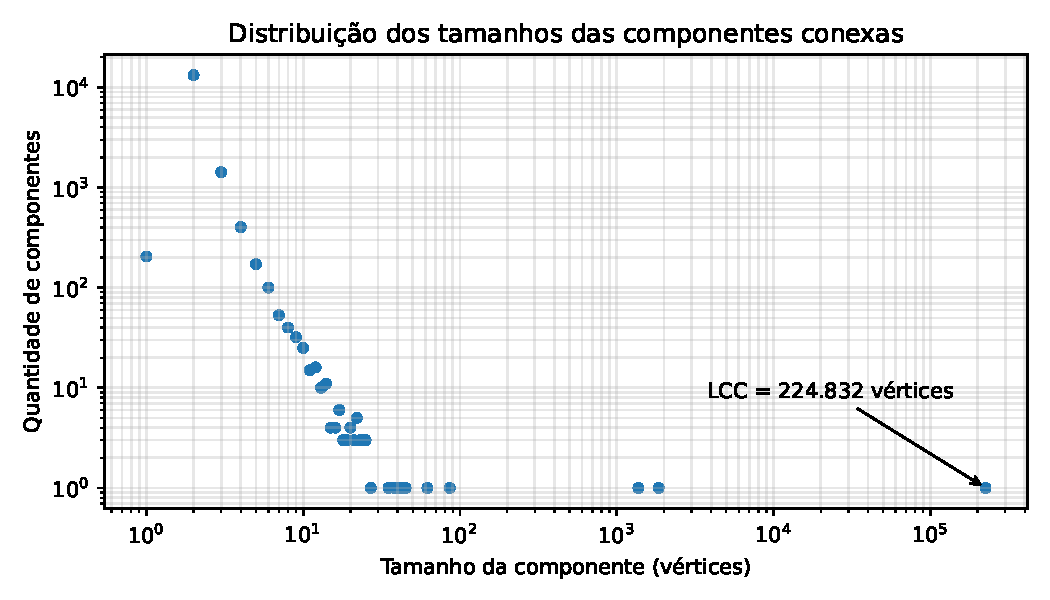
\includegraphics[width=\linewidth]{componentes_tamanhos}
  \caption{Quantidade de componentes conexas por tamanho (log-log). Há uma única componente gigante e milhares de componentes pequenas.}
  \Description{Gráfico de dispersão em escala log-log: o número de componentes cai rapidamente com o tamanho; isolada à direita, a componente gigante de 224.832 vértices.}
  \label{fig:componentes}
\end{figure}

\textbf{Distâncias.} O diâmetro é 14 e o raio é 7, ambos exatos. O comprimento médio
estimado é $L = 4{,}127$ (IC 95\%: $[4{,}098;\,4{,}156]$, 500 fontes). A estimativa com
100 fontes (4,118; IC $[4{,}037;\,4{,}199]$) é consistente com ela, o que indica que o
estimador é estável. Assim, dois endereços quaisquer da LCC estão, em média, a pouco mais
de 4 saltos de distância, apesar dos 224 mil vértices.

\textbf{Clusterização.} Há 267.313 triângulos, envolvendo 25.132 vértices. A
clusterização média ($C=0{,}079$) é cerca de 19 vezes maior que a transitividade
($0{,}0042$). Isso ocorre porque a transitividade é dominada pelos hubs, cujos milhares
de vizinhos quase nunca se conectam entre si, enquanto a média local é puxada por
vértices de grau baixo inseridos em grupos coesos.

\textbf{Distribuição de graus e visualização.} A Figura~\ref{fig:graus} mostra a
concentração em graus baixos (escala linear) e o decaimento aproximadamente linear em
escala log-log, analisado na Parte~III. A Figura~\ref{fig:visualizacao} desenha uma
amostra de 300 vértices em torno dos 5 maiores hubs e revela dois padrões: o maior hub é
uma \emph{estrela} quase pura, ligada a vértices de grau 1, enquanto os vizinhos de grau
alto dos demais hubs formam um núcleo denso.

\begin{figure*}[t]
  \centering
  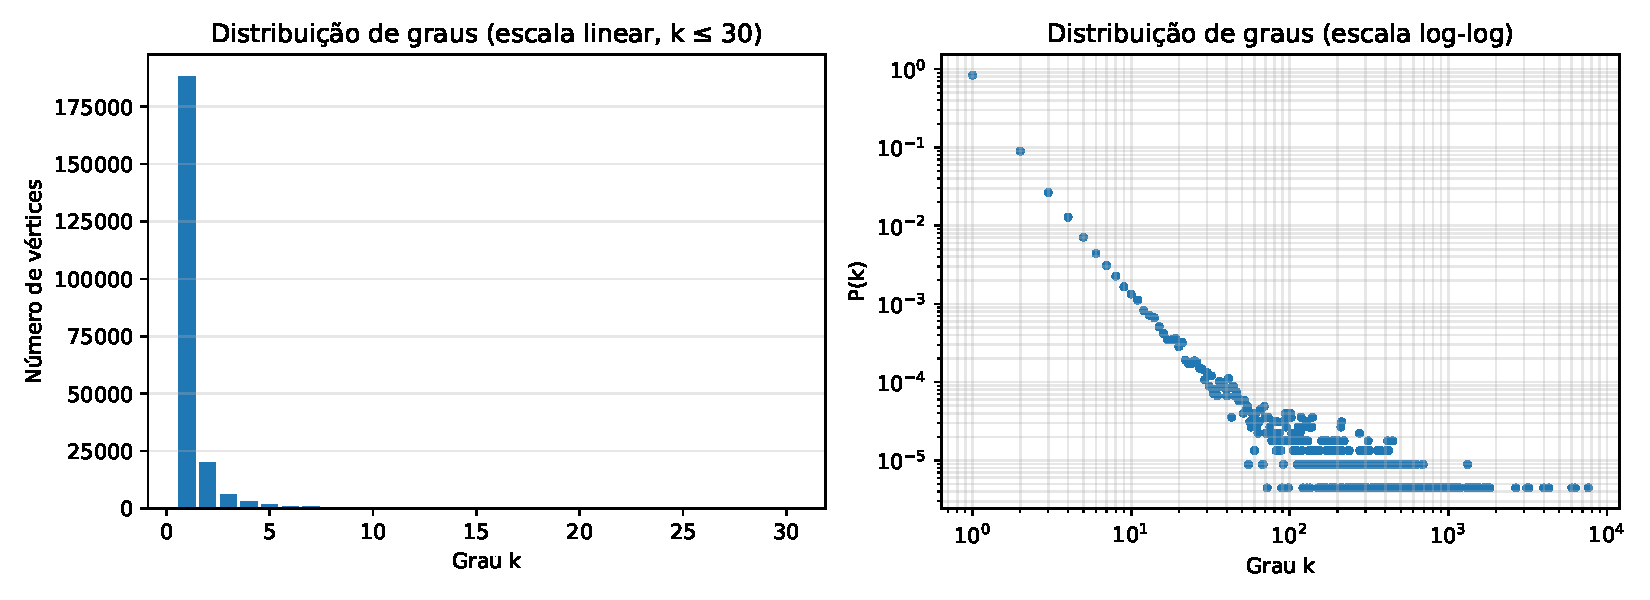
\includegraphics[width=0.85\textwidth]{distribuicao_graus}
  \caption{Distribuição de graus da LCC em escala linear, para $k \le 30$ (esquerda), e em escala log-log (direita).}
  \Description{À esquerda, barras mostrando cerca de 188 mil vértices de grau 1 e quedas rápidas para graus maiores. À direita, P(k) em log-log decaindo aproximadamente em linha reta, com uma faixa de pontos dispersos na cauda.}
  \label{fig:graus}
\end{figure*}

\begin{figure}[t]
  \centering
  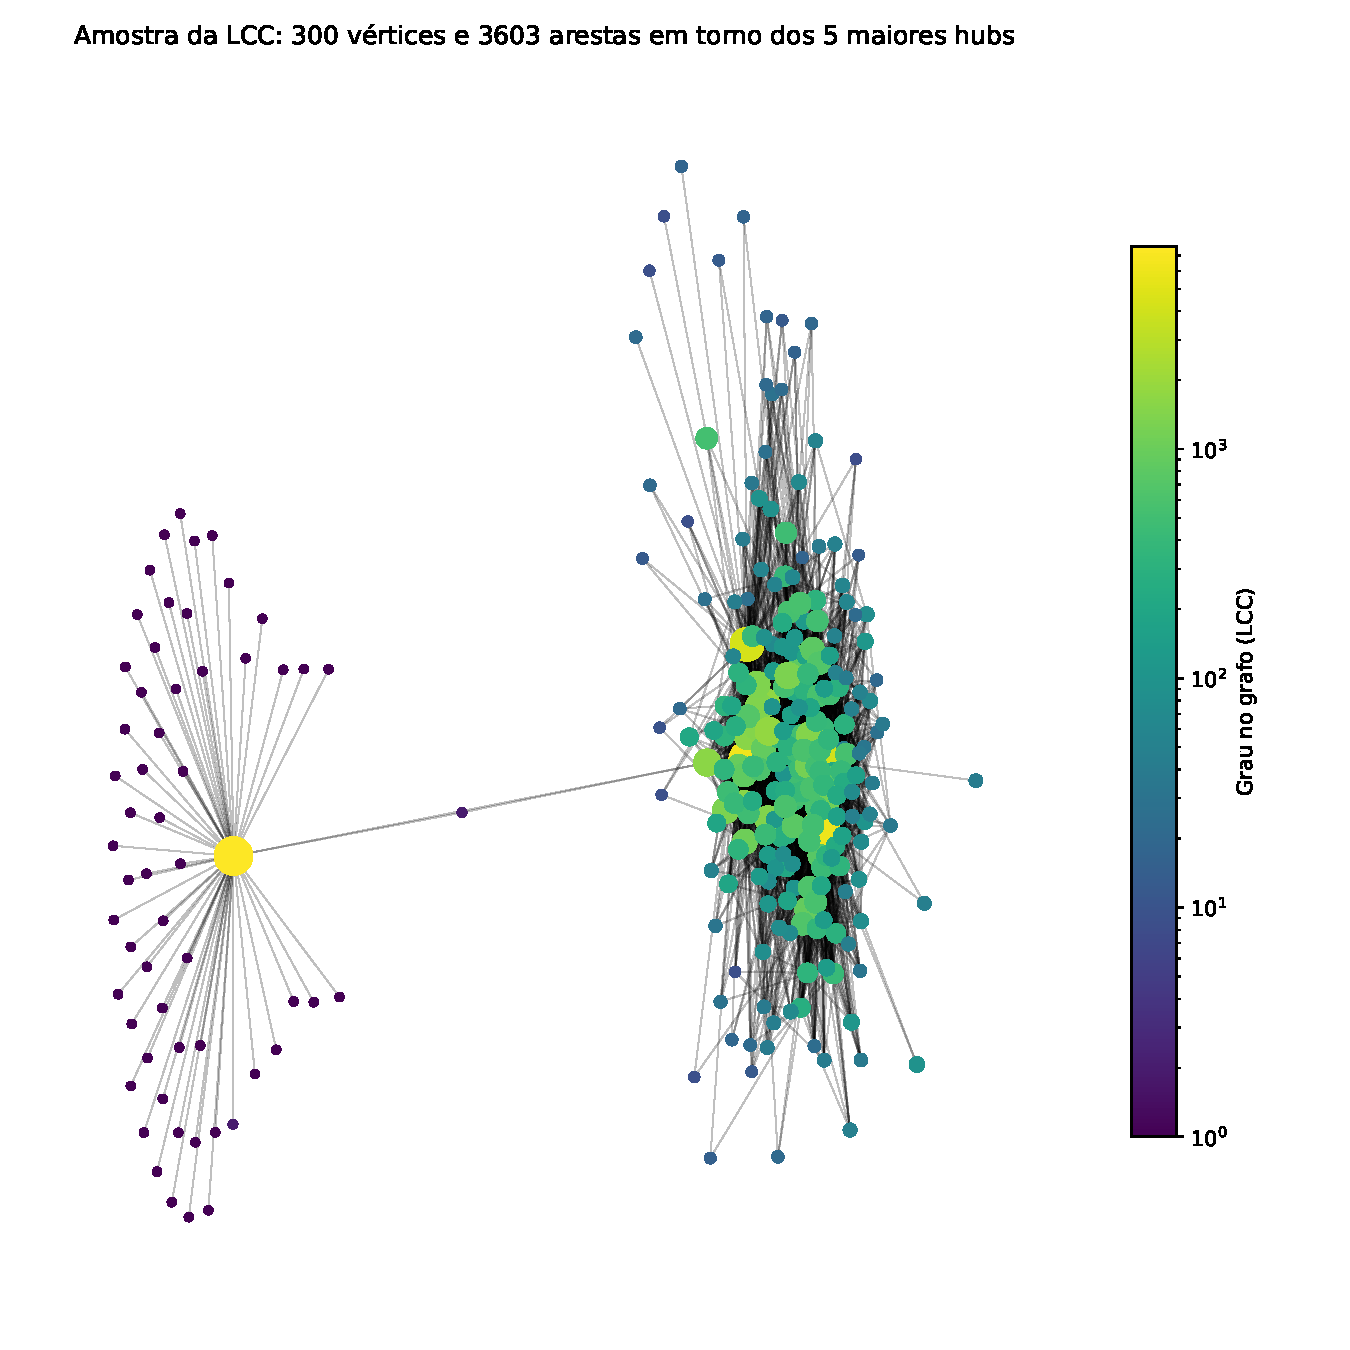
\includegraphics[width=0.95\linewidth]{visualizacao_amostra}
  \caption{Amostra de 300 vértices da LCC em torno dos 5 maiores hubs (cor e tamanho proporcionais ao grau). O maior hub (à esquerda) forma uma estrela, e os demais compõem um núcleo denso.}
  \Description{Desenho de grafo: à esquerda, um vértice amarelo grande ligado a dezenas de folhas roxas; à direita, um aglomerado denso de vértices de grau alto; um único caminho curto liga as duas partes.}
  \label{fig:visualizacao}
\end{figure}

\subsection{Parte II: Algoritmos da Disciplina}

A Tabela~\ref{tab:algoritmos} resume, para cada algoritmo, o grafo em que foi executado,
a complexidade teórica, o tempo observado (média, desvio e IC 95\%) e o resultado.

% Gerado por src/report_tables.py a partir de results/tables/ -- não editar
\begin{table*}[t]
  \caption{Algoritmos: complexidade teórica, tempo observado e resultado. IC 95\% pela Normal ($n=30$), exceto onde indicado com * (t-Student, $n=10$).}
  \label{tab:algoritmos}
\resizebox{\textwidth}{!}{%
\begin{tabular}{llllrrl}
  \toprule
  Algoritmo & Grafo & Complexidade & Média (s) & Desvio (s) & IC 95\% (s) & Resultado \\
  \midrule
  BFS & LCC & $O(V+E)$ & 0,1980 & 0,0425 & [0,1828; 0,2132] & visitou 224.832 vértices; profundidade máx. 10 \\
  DFS (iterativa) & LCC & $O(V+E)$ & 0,3195 & 0,0093 & [0,3162; 0,3228] & visitou 224.832 vértices \\
  Eulerianidade (não dirigido) & LCC & $O(V+E)$ & 0,1658 & 0,0031 & [0,1647; 0,1669] & não euleriano; 198.520 vértices de grau ímpar \\
  Eulerianidade (dirigido) & $G_{dir}$ & $O(V+E)$ & 0,5057 & 0,0050 & [0,5039; 0,5075] & não euleriano; 242.614 vértices com entrada$\neq$saída; fracamente conexo: não \\
  Dijkstra (heap) & LCC ponderada & $O((V+E)\log V)$ & 0,7703 & 0,0101 & [0,7667; 0,7740] & alcançou 224.832 vértices; dist. máx. 41 \\
  Bellman-Ford & subgrafo 300 & $O(V\cdot E)$ & 0,0003 & 0,0000 & [0,0003; 0,0003] & alcançou 300 vértices; 3 rodadas \\
  Floyd-Warshall (Python puro)* & subgrafo 300 & $O(V^3)$ & 1,9521 & 0,0170 & [1,9400; 1,9643] & matriz 300$\times$300; dist. máx. 20 \\
  Floyd-Warshall (numpy) & subgrafo 300 & $O(V^3)$ & 0,0570 & 0,0013 & [0,0566; 0,0575] & matriz 300$\times$300; dist. máx. 20 \\
  Tarjan (SCC) & $G_{dir}$ & $O(V+E)$ & 0,6071 & 0,0114 & [0,6031; 0,6112] & 231.000 SCCs; maior com 34.203 vértices \\
  Tarjan (pontes/articulações) & LCC & $O(V+E)$ & 0,5771 & 0,0236 & [0,5686; 0,5855] & 188.668 pontes; 2.223 articulações \\
  Prim (heap) & LCC ponderada & $O(E\log V)$ & 0,9036 & 0,0184 & [0,8970; 0,9102] & 224.831 arestas; peso total 1.151.996 \\
  Kruskal (union-find) & LCC ponderada & $O(E\log V)$ & 0,5255 & 0,0082 & [0,5226; 0,5285] & 224.831 arestas; peso total 1.151.996 \\
  \bottomrule
\end{tabular}}
\end{table*}


\textbf{BFS e DFS.} Ambas visitaram os 224.832 vértices, confirmando que a LCC é
conexa. A BFS a partir do vértice 0 atinge profundidade 10, sua excentricidade. A DFS é
mais lenta por manter, para cada vértice da pilha, o índice do próximo vizinho, o que
reproduz exatamente a ordem da DFS recursiva.

\textbf{Eulerianidade.} Pelo teorema de Euler, um grafo conexo tem circuito euleriano
se todos os graus são pares, e caminho euleriano se exatamente dois graus são ímpares.
A LCC tem 198.520 vértices de grau ímpar e, portanto, não é euleriana. No dirigido,
242.614 vértices têm grau de entrada diferente do de saída, e o grafo nem é fracamente
conexo. Também implementamos o algoritmo de Hierholzer, que constrói o circuito quando
ele existe (validado nos testes).

\textbf{Dijkstra e Bellman-Ford.} Os dois se aplicam porque os pesos sintéticos são
positivos. Com peso unitário, Dijkstra equivaleria à BFS. Dijkstra alcançou toda a LCC
e foi cerca de 4 vezes mais lento que a BFS, devido ao custo do heap. Bellman-Ford
($O(V\cdot E)$) foi executado apenas no subgrafo: na LCC seriam até
$224.832 \times 679.850 \approx 1{,}5\times10^{11}$ relaxamentos no pior caso. Ele produziu
as mesmas distâncias que Dijkstra e parou após apenas 3 das até $V-1=299$ rodadas, graças à
parada antecipada: como cada rodada percorre todas as arestas em sequência, uma única
rodada pode propagar distâncias por vários saltos. Para não depender só desse subgrafo,
ele também foi medido em subgrafos de até 16 mil vértices no estudo de escala, a seguir.
Não havendo pesos negativos, Dijkstra é preferível nesse contexto.

\textbf{Floyd-Warshall.} No subgrafo de 300 vértices, a versão em Python puro levou
1,95~s e a vetorizada (numpy, mesmo algoritmo $O(V^3)$) levou 0,057~s, 34 vezes menos. O
resultado confere com Dijkstra executado a partir de todas as 300 fontes. Na LCC seriam
$\approx1{,}1\times10^{16}$ operações e uma matriz de $5\times10^{10}$ células (cerca de
400~GB), o que é inviável.

\textbf{Tarjan.} Na versão dirigida, a maior componente fortemente conexa tem apenas
34.203 vértices (12,9\%), enquanto a maior componente não dirigida tem 84,8\%: a maior
parte da comunicação não é recíproca. Com a mesma técnica de \emph{low-link} obtivemos
188.668 pontes (quase todas arestas de folhas) e 2.223 vértices de articulação na LCC.

\textbf{Prim e Kruskal.} Ambos produziram árvores com $V-1 = 224.831$ arestas e o mesmo
peso total (1.151.996), o que confirma a correção. Kruskal foi mais rápido: a ordenação
das 339.925 arestas é feita em C pelo Python, e o \emph{union-find} com compressão de
caminho e união por rank tem custo quase constante.

\textbf{Complexidade observada.} A Figura~\ref{fig:tempos} compara os tempos médios. Para
estudar o crescimento, medimos \emph{os nove algoritmos} em subgrafos de tamanho
crescente, induzidos por prefixos da ordem de BFS da LCC (todos conexos). Os de custo
linear ou quase linear foram medidos de 14 mil vértices até a LCC inteira; Bellman-Ford,
de 1 mil a 16 mil; e Floyd-Warshall, de 50 a 300. Foram 30 repetições por tamanho, com
IC 95\% (Normal) em cada ponto. Em cada painel da Figura~\ref{fig:escala}, o tempo é
ajustado em log-log contra a própria função teórica $f(n)$: se ela descreve o custo, a
inclinação é 1 (Tabela~\ref{tab:escala}).

Floyd-Warshall (1,00 contra $V^3$, $R^2=0{,}9998$), Tarjan (0,98), Kruskal (1,05) e Prim
(1,06) confirmam a teoria. \textbf{Bellman-Ford} ficou muito abaixo do pior caso
(0,61 contra $V\cdot E$): com a parada antecipada, ele convergiu em apenas 4 ou 5 rodadas
em todos os tamanhos. Seu custo real foi, portanto, $O(k\cdot E)$ com $k$ pequeno, e não
$O(V\cdot E)$, porque a cota de $V-1$ rodadas só é atingida em grafos com caminhos mínimos
muito longos.

BFS (1,49), Eulerianidade (1,31), Dijkstra (1,31) e DFS (1,27) cresceram mais rápido que
o previsto, com ICs estreitos e $R^2 \ge 0{,}99$, ou seja, não é ruído de medição. O
número de operações é linear: os testes confirmam que cada vértice entra uma única vez
na fila ou na pilha. O que cresce é o custo de cada operação. Como o Tarjan percorre as
mesmas listas de adjacência e ficou em 0,98, o tamanho do grafo sozinho não explica o
desvio. Atribuímos o restante a efeitos do interpretador Python, como a alocação de
listas de tamanho $V$ e o gerenciamento de memória, que variam entre implementações.
Essa é uma hipótese, não algo que tenhamos isolado. A faixa testada, de pouco mais de uma
ordem de grandeza, também limita a precisão do expoente.

% Gerado por src/report_tables.py a partir de results/tables/ -- não editar
\begin{table}[t]
  \caption{Complexidade observada: inclinação em log-log do tempo médio contra o tamanho da entrada e contra a função teórica $f(n)$ (ideal: 1).}
  \label{tab:escala}
\resizebox{\columnwidth}{!}{%
\begin{tabular}{lrrrlrr}
  \toprule
  Algoritmo & Teórico & Observado & $R^2$ & $f(n)$ & Exp. vs.\ $f$ & $R^2$ \\
  \midrule
  BFS & 1 & 1,50 & 0,995 & $V+E$ & 1,50 & 0,995 \\
  Dijkstra & 1 & 1,53 & 0,993 & $(V+E)\log V$ & 1,36 & 0,994 \\
  Floyd-Warshall & 3 & 2,98 & 1,000 & $V^3$ & 0,99 & 1,000 \\
  \bottomrule
\end{tabular}}
\end{table}


\begin{figure}[t]
  \centering
  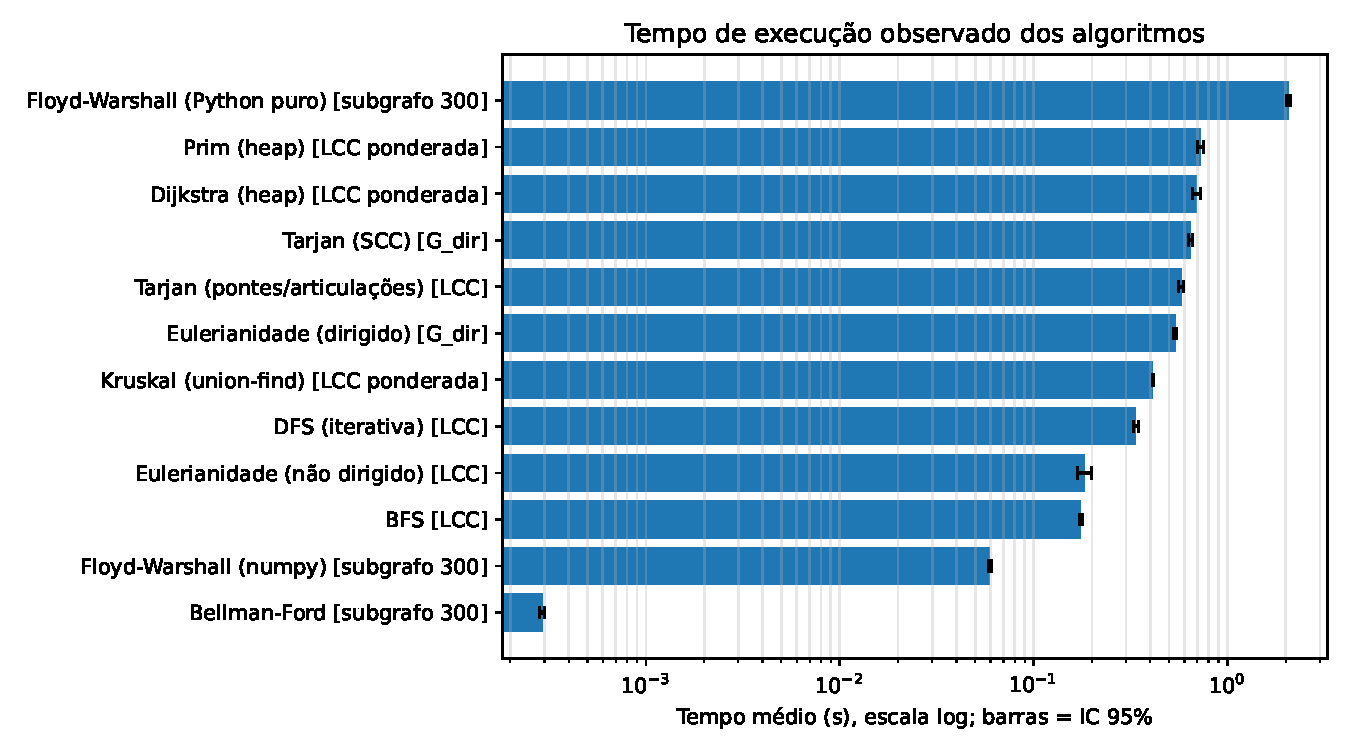
\includegraphics[width=\linewidth]{tempos_algoritmos}
  \caption{Tempo médio de cada algoritmo (escala log; barras de erro = IC 95\%).}
  \Description{Gráfico de barras horizontais em escala logarítmica, do Bellman-Ford (mais rápido, no subgrafo) ao Floyd-Warshall em Python puro (mais lento).}
  \label{fig:tempos}
\end{figure}

\begin{figure*}[t]
  \centering
  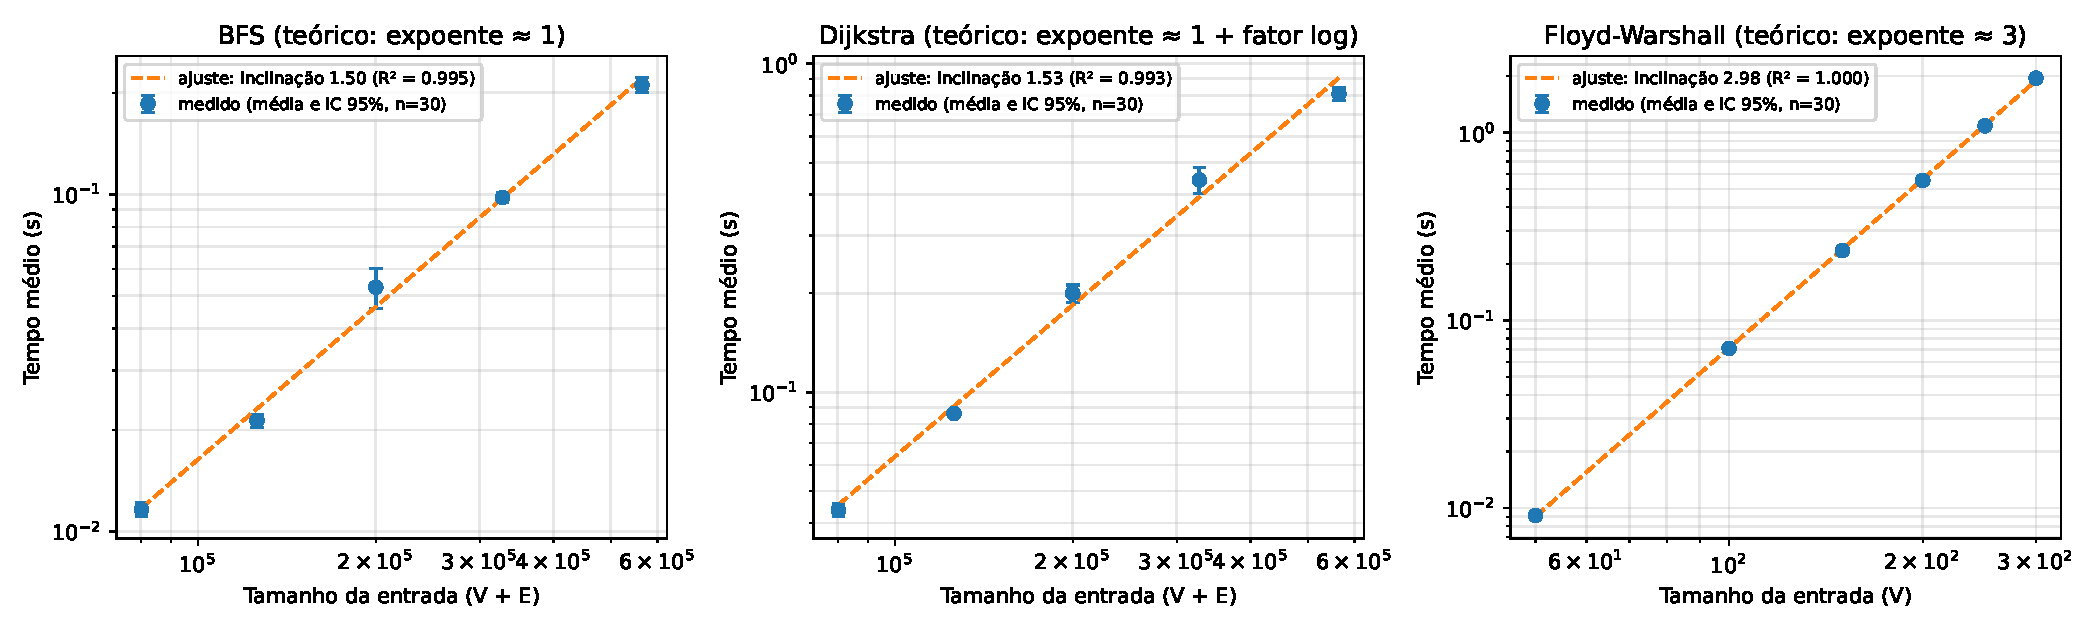
\includegraphics[width=\textwidth]{escala_algoritmos}
  \caption{Complexidade observada dos nove algoritmos: tempo médio (IC 95\%, 30 repetições por tamanho) contra a função teórica $f(n)$, em log-log. Inclinação 1 indica que $f(n)$ descreve o custo observado.}
  \Description{Nove gráficos log-log, um por algoritmo, com pontos alinhados sobre retas ajustadas. As inclinações vão de 0,61 (Bellman-Ford) a 1,49 (BFS); Floyd-Warshall, Tarjan, Prim e Kruskal ficam próximos de 1.}
  \label{fig:escala}
\end{figure*}

\subsection{Parte III: Análise de Propriedades da Rede}

\subsubsection{Small-world}
Seguindo o Apêndice~A~\cite{watts1998,humphries2008}, comparamos $L$ e $C$ da LCC com
uma referência aleatória de Erd\H{o}s--Rényi $G(n,m)$~\cite{erdos1959} com o mesmo número de
vértices e de arestas (logo o mesmo $\langle k \rangle = 3{,}024$), gerada por código
próprio, sem bibliotecas prontas, em 5 realizações. Como o $G(n,m)$ com
$\langle k\rangle\approx3$ não é conexo, $L_{rand}$ foi medido na sua maior componente
(94,2\% dos vértices). Os valores analíticos
$C_{rand}\approx\langle k\rangle/n$ e $L_{rand}\approx\ln n/\ln\langle k\rangle$ servem
de conferência. O coeficiente é $\sigma = (C/C_{rand})/(L/L_{rand})$, e $\sigma > 1$
indica \emph{small-world}.

% Gerado por src/report_tables.py a partir de results/tables/ -- não editar
\begin{table}[t]
  \caption{Small-world: grafo real (LCC, $L$ exato) contra dois modelos nulos: Erd\H{o}s--Rényi equivalente (média de 5 realizações, e valores analíticos) e reconexão que preserva os graus (média de 3 realizações).}
  \label{tab:smallworld}
\resizebox{\columnwidth}{!}{%
\begin{tabular}{lrrrr}
  \toprule
  Métrica & Real & ER medido & ER analítico & Graus preservados \\
  \midrule
  $L$ & 4,118 & 11,116 & 11,137 & 3,624 \\
  $C$ & 0,0791 & $7{,}8\times10^{-6}$ & $1{,}3\times10^{-5}$ & 0,0337 \\
  $C/C_{nulo}$ & -- & $\approx$ 10.142 & $\approx$ 5.884 & 2,35 \\
  $L/L_{nulo}$ & -- & 0,370 & 0,370 & 1,136 \\
  $\sigma$ & -- & $\approx$ 27.375 & $\approx$ 15.912 & 2,07 \\
  \bottomrule
\end{tabular}}
\end{table}


\textbf{O grafo é small-world? Sim, de forma inequívoca} (Tabela~\ref{tab:smallworld}). A
clusterização é cerca de 10 mil vezes maior que a do grafo aleatório equivalente, e o
comprimento médio dos caminhos é até \emph{menor} que o aleatório (4,1 contra 11,1),
pois os hubs funcionam como atalhos que o $G(n,m)$, de grau quase homogêneo, não tem.
\textbf{Faz sentido para este grafo:} e-mails institucionais formam grupos coesos
(equipes, departamentos), o que explica o $C$ alto, e alguns endereços centrais (listas,
secretarias, servidores) ligam os grupos, o que explica o $L$ baixo. \textbf{Implicação
prática:} informação, boatos, vírus ou spam se espalham para quase toda a rede em
poucos saltos, e a mesma estrutura permite contatar qualquer membro por poucos
intermediários.

\subsubsection{Lei de potência}
Seguindo o Apêndice~B, calculamos o grau de cada vértice, a frequência de cada valor de
$k$, o histograma $P(k)$ e a CCDF $P(K\ge k)$ em escala log-log
(Figura~\ref{fig:powerlaw}). Para ajuste, usamos: (i) regressão linear em log-log de $P(k)$
com \emph{log-binning}; (ii) regressão na CCDF, cuja inclinação é $-(\gamma-1)$; e (iii)
máxima verossimilhança discreta~\cite{clauset2009}, com $k_{min}$ escolhido pela
distância de Kolmogorov--Smirnov (KS). A Tabela~\ref{tab:powerlaw} resume os resultados.

% Gerado por src/report_tables.py a partir de results/tables/ -- não editar
\begin{table}[t]
  \caption{Estimativas do expoente $\gamma$ de $P(k)\sim k^{-\gamma}$ (LCC).}
  \label{tab:powerlaw}
\resizebox{\columnwidth}{!}{%
\begin{tabular}{lrl}
  \toprule
  Método & $\gamma$ & Observação \\
  \midrule
  Regressão $P(k)$, log-binning & 1,94 & $R^2 = 0{,}983$ \\
  Regressão na CCDF & 2,03 & $R^2 = 0{,}904$ \\
  MLE, $k_{min}=1$ (cabeça) & 2,83 & KS = 0,031 \\
  MLE, $k_{min}=9$ (cauda) & 1,74 & KS = 0,052; 3.762 vértices \\
  \bottomrule
\end{tabular}}
\end{table}


\begin{figure*}[t]
  \centering
  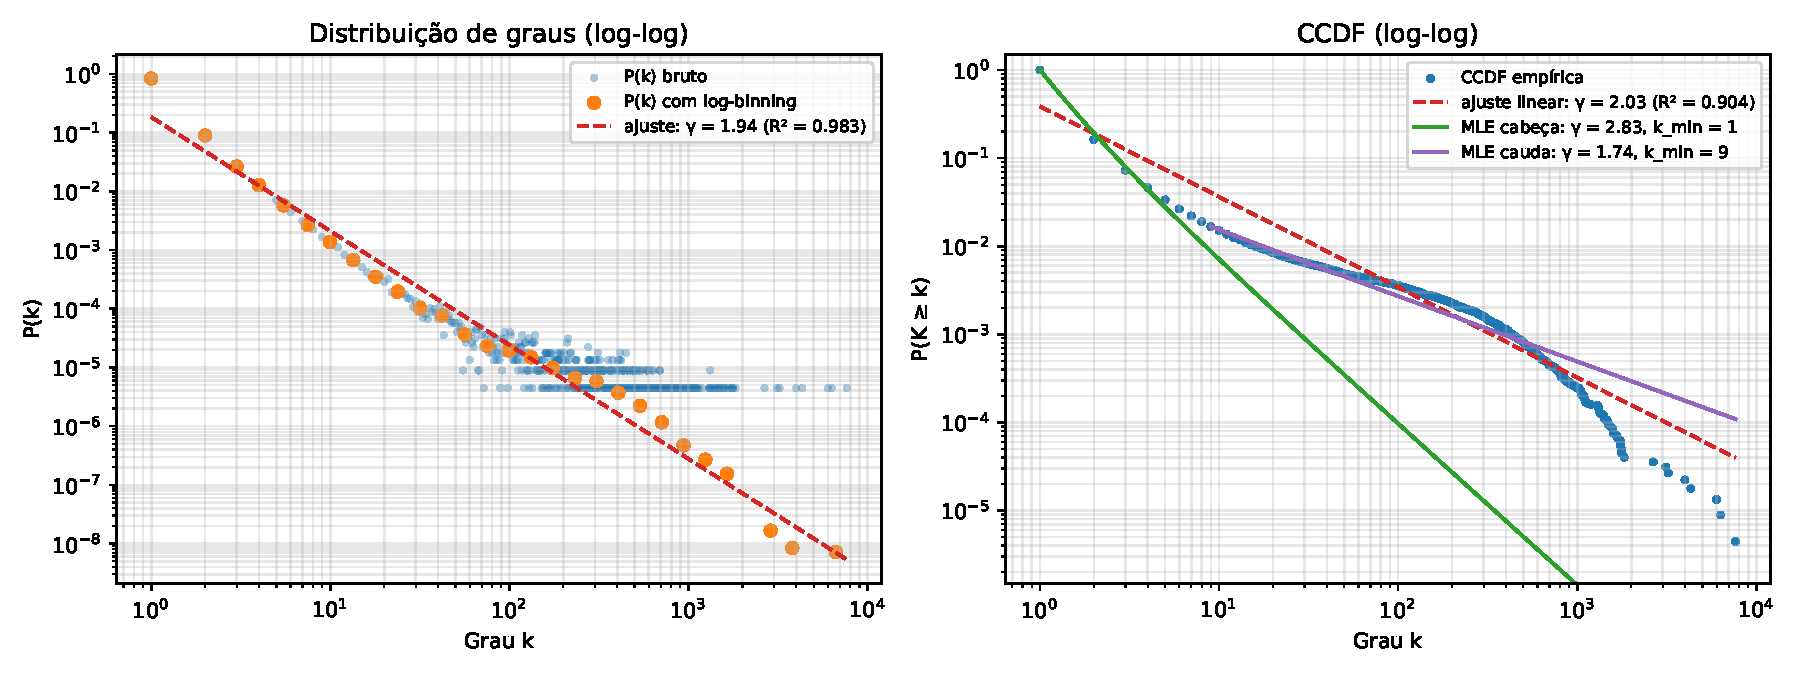
\includegraphics[width=0.9\textwidth]{lei_de_potencia}
  \caption{Distribuição de graus em log-log com log-binning e ajuste linear (esquerda) e CCDF com ajustes linear e por máxima verossimilhança para a cabeça e para a cauda (direita).}
  \Description{À esquerda, P(k) em log-log quase linear com inclinação de cerca de -1,94. À direita, a CCDF mostra uma queda íngreme até k=10, um trecho mais plano até cerca de k=500 e uma queda acentuada depois de k=1000.}
  \label{fig:powerlaw}
\end{figure*}

\textbf{A distribuição sugere lei de potência? Apenas aproximadamente.} O histograma em
log-log é quase uma reta ($R^2=0{,}98$, $\gamma\approx1{,}9$), e a cauda é claramente
pesada: hubs de grau até 7.636 seriam virtualmente impossíveis numa distribuição de
Poisson com média 3. A CCDF, porém, mostra \emph{dois regimes} e um corte: uma queda
íngreme na cabeça ($\gamma\approx2{,}8$, dominada pelos 84\% de vértices de grau 1),
uma cauda mais plana entre $k\approx10$ e $k\approx500$ ($\gamma\approx1{,}7$) e uma
queda acentuada acima de $k\approx1.000$. A estimativa de máxima verossimilhança varia
de 2,83 a 1,66 conforme $k_{min}$, e a distância KS na cauda (0,05 a 0,13) é alta. A
conclusão é que a rede é livre de escala no sentido qualitativo (heterogênea, com
hubs), mas uma lei de potência pura não descreve bem toda a distribuição.

\subsubsection{Robustez}
Seguindo o Apêndice~C, trabalhamos na LCC ($N = 224.832$) e removemos
$r=\lfloor0{,}05N\rfloor=11.241$ vértices em dois cenários: (a) remoção aleatória,
com $R=30$ repetições; e (b) ataque direcionado pelo \emph{ranking fixo} de uma
centralidade, calculado uma vez no grafo original, removendo os $r$ primeiros. Usamos
duas das centralidades recomendadas: o \textbf{grau}, que remove os hubs, e o
\textbf{PageRank}, que mede influência global. O PageRank foi implementado por iteração
de potência, com amortecimento $d=0{,}85$, convergiu em 129 iterações e foi validado
contra o NetworkX. A betweenness exata não foi usada por custar
$O(V\cdot E)\approx7{,}6\times10^{10}$ operações. As métricas são: A, a fração $S/N$ de
vértices na maior componente; B, o número de componentes; C, o comprimento médio na
maior componente (50 fontes); e D, a fração de vértices isolados entre os restantes.

% Gerado por src/report_tables.py a partir de results/tables/ -- não editar
\begin{table}[t]
  \caption{Robustez após remover 5\% dos vértices (média $\pm$ desvio em 30 repetições na remoção aleatória; ataques com ranking fixo).}
  \label{tab:robustez}
\resizebox{\columnwidth}{!}{%
\begin{tabular}{lrrrrr}
  \toprule
  Métrica & Original & Aleatória & Ataque: Grau & Ataque: PageRank & Ataque: Betweenness \\
  \midrule
  A: $S/N$ & 1 & $0{,}907 \pm 0{,}017$ & $2{,}67\times10^{-5}$ & $1{,}33\times10^{-5}$ & $4{,}89\times10^{-5}$ \\
  B: componentes & 1 & $9.431 \pm 3.486$ & 213.168 & 213.396 & 213.264 \\
  C: $L$ (maior comp.) & 4,02 & $4{,}12 \pm 0{,}04$ & 1,93 & 1,33 & 2,29 \\
  D: isolados & 0,000 & $0{,}044 \pm 0{,}016$ & 0,997 & 0,998 & 0,998 \\
  \bottomrule
\end{tabular}}
\end{table}


\begin{figure*}[t]
  \centering
  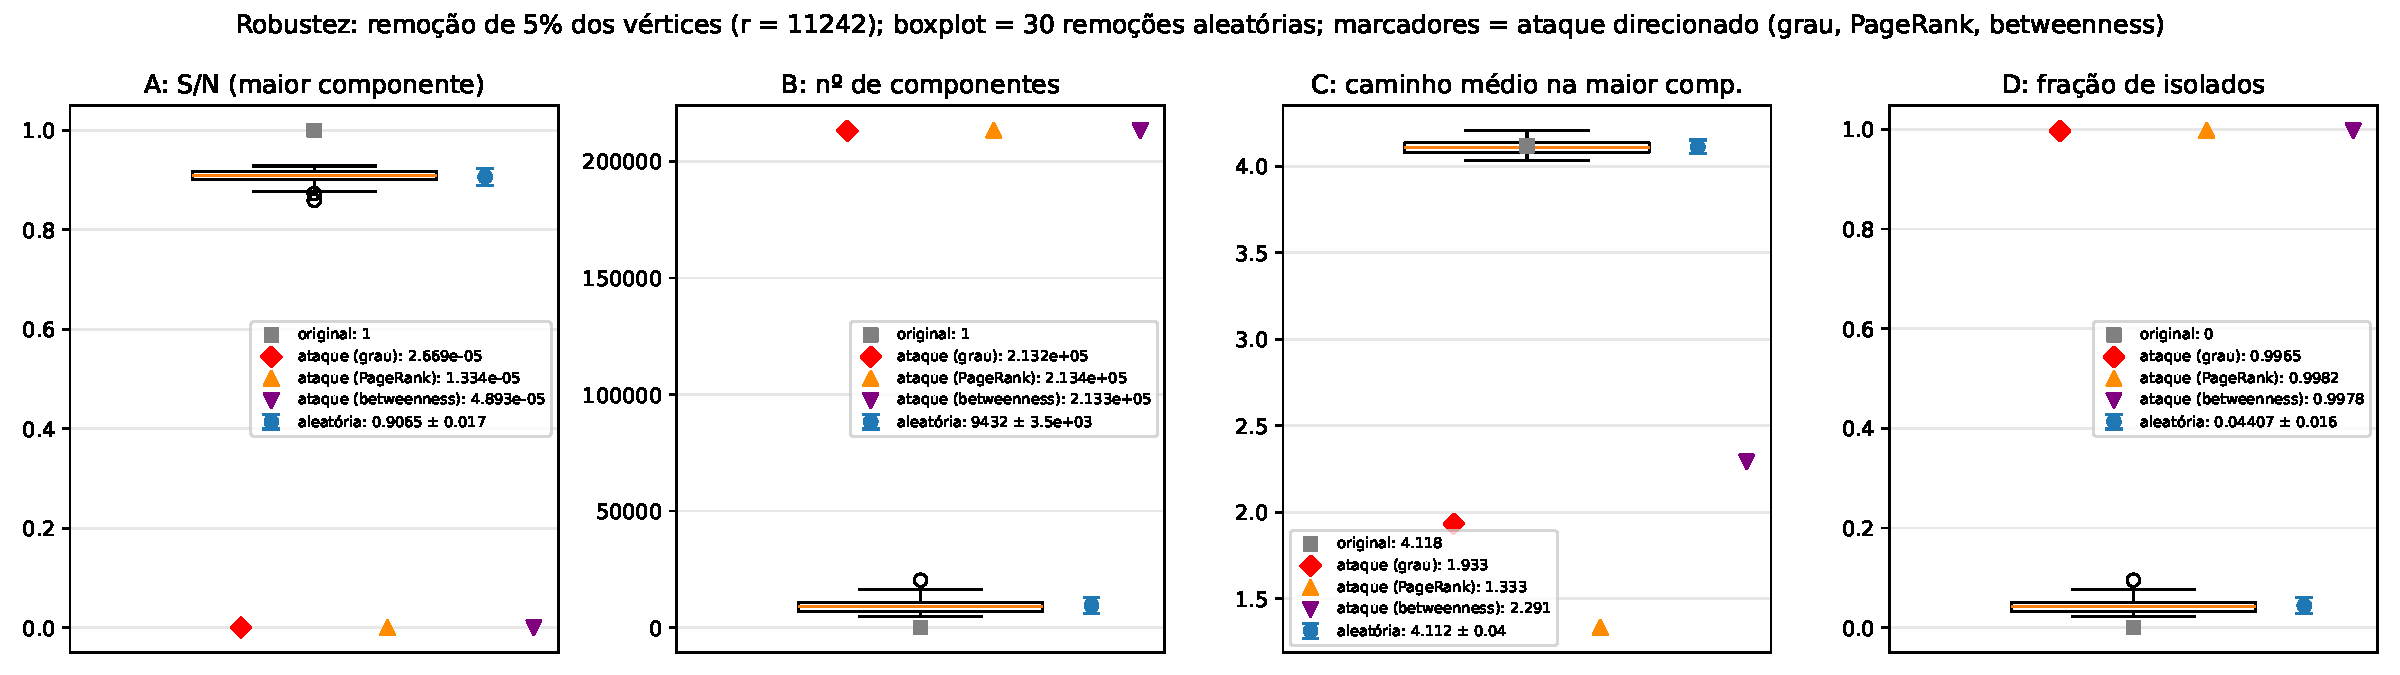
\includegraphics[width=\textwidth]{robustez}
  \caption{Métricas A a D após remover 5\% dos vértices: boxplots das 30 remoções aleatórias (com média $\pm$ desvio em azul), valor original (quadrado cinza) e ataques aos vértices de maior grau (losango vermelho) e de maior PageRank (triângulo laranja).}
  \Description{Quatro painéis. Nos painéis A e D, os boxplots aleatórios ficam próximos do original (0,9 e 0,04), enquanto os marcadores dos dois ataques estão no extremo oposto (cerca de 0 e 1). No painel B, os ataques geram mais de 200 mil componentes, contra cerca de 9 mil na remoção aleatória.}
  \label{fig:robustez}
\end{figure*}

\textbf{(a) Robusta à remoção aleatória de 5\%? Sim.} A maior componente mantém
$S_{rand}/S_0 = 0{,}907$ dos vértices (Tabela~\ref{tab:robustez} e
Figura~\ref{fig:robustez}): perde pouco mais que os 5\% removidos. O comprimento médio
quase não muda (4,02 para 4,12), e só 4,4\% dos vértices ficam isolados. O desvio
alto de B (cerca de 3.500) ocorre porque, quando o sorteio atinge um hub por acaso, suas
folhas se desprendem.

\textbf{(b) Robusta à remoção dos 5\% mais centrais? Não, por nenhuma das duas
centralidades.} No ataque por grau, $S_{target}/S_0 = 2{,}7\times10^{-5}$: a maior
componente restante tem \textbf{6 vértices}, há 213.168 componentes e 99,7\% dos
vértices restantes ficam isolados. O ataque por PageRank é ainda um pouco mais
destrutivo: a maior componente fica com \textbf{3 vértices}
($S_{target}/S_0 = 1{,}3\times10^{-5}$) e 99,8\% dos vértices ficam isolados. As duas
centralidades escolhem quase os mesmos alvos (93\% de sobreposição entre os top-$r$),
porque, nesta rede, influência global e número de contatos andam juntos. Os valores
1,93 e 1,33 de C não indicam melhora: são distâncias médias
dentro de ``componentes'' de 6 e 3 vértices. Como $S_{target} \ll S_{rand}$, a rede é
extremamente vulnerável a ataques direcionados, padrão típico de redes com hubs e cauda
pesada~\cite{albert2000}.

\subsubsection{Descoberta mais interessante}
A descoberta mais interessante foi \textbf{quão pouco da rede é ``de verdade'' uma rede}.
A conectividade de 224 mil endereços depende quase só dos hubs. Os 5 maiores hubs têm
de 94\% a 100\% dos vizinhos com grau 1: são estrelas, ligando milhares de endereços que
trocaram e-mail com uma única pessoa. Além disso, 72\% dos vértices aparecem
\emph{apenas} como origem de mensagens, só 26\% das arestas são recíprocas, e a maior
componente fortemente conexa tem apenas 12,9\% dos vértices: exatamente os 34.203
endereços que, segundo o SNAP, enviaram \emph{e} receberam mensagens. O quadro é o de um
núcleo pequeno de 1.258 endereços da instituição, que se comunicam entre si, cercado por
uma periferia enorme de endereços externos que o SNAP descreve como inexistentes,
digitados incorretamente ou de spam. Essa estrutura explica, ao mesmo tempo, o $L$
baixo, a cauda pesada e o colapso completo quando os 5\% de maior grau, que concentram
64\% das extremidades de arestas, são removidos. Na prática, a ``rede de 224 mil
endereços'' é, sobretudo, o tráfego de e-mail de pouco mais de mil pessoas.

\subsubsection{Extra: aproximação a modelos clássicos}
Não simulamos os modelos, mas as medidas permitem uma comparação qualitativa. O
\textbf{Erd\H{o}s--Rényi} é descartado: tem graus aproximadamente Poisson, $C$ cerca de 10
mil vezes menor e $L$ quase três vezes maior (Tabela~\ref{tab:smallworld}). O
\textbf{Watts--Strogatz} reproduz $C$ alto e $L$ baixo, mas tem graus homogêneos e não
gera hubs de grau 7.636. O \textbf{Barabási--Albert}~\cite{barabasi1999} é o mais próximo
pela cauda pesada e pela fragilidade a ataques, mas prevê $\gamma=3$, nenhum vértice com
grau abaixo de $m$ e $C\to0$ em redes grandes, enquanto aqui 84\% dos vértices têm grau 1
e $C=0{,}079$. A rede combina características de BA (hubs) e WS (agrupamento), sem se
reduzir a nenhum dos dois.

%% ===================================================================
\section{Discussão Crítica}
\label{sec:discussao}

\textbf{Decisões de tratamento.} A conversão para não dirigido é adequada às perguntas
de conectividade, mas apaga a assimetria da comunicação, que é justamente uma das
características mais marcantes da rede (26\% de reciprocidade). Por isso mantivemos o
grafo dirigido para o Tarjan. Trabalhar na LCC descarta 15,2\% dos vértices, em sua
maioria pares ou trincas isolados, que pouco influenciam as conclusões.

\textbf{Exatidão contra aproximação.} Diâmetro e raio foram obtidos de forma exata com
apenas 4 BFS, o que mostra que a escolha de algoritmo pode tornar viável um cálculo
que parecia exigir $10^{11}$ operações. O comprimento médio permaneceu amostral, mas
com IC estreito e estável entre 100 e 500 fontes.

\textbf{Pesos sintéticos.} Dijkstra, Bellman-Ford, Floyd-Warshall e as árvores
geradoras usam pesos aleatórios que não têm significado no domínio. Os resultados
servem para validar e medir os algoritmos, não para interpretar a rede. Pesos reais,
como o número de mensagens por par, não estão disponíveis no dataset.

\textbf{Tempos em Python.} A diferença de 34 vezes entre as duas versões do
Floyd-Warshall, com a mesma complexidade, mostra que o tempo real depende fortemente
de constantes de implementação. O estudo de escala reforça a lição em dois sentidos: o
Bellman-Ford, com parada antecipada, ficou muito abaixo do seu pior caso $O(V\cdot E)$,
e algoritmos lineares como BFS e DFS cresceram acima do previsto. A complexidade
assintótica conta operações no pior caso, não o custo real de cada operação nem o
comportamento em instâncias típicas.

\textbf{Lei de potência.} Ajustes lineares em log-log produzem retas convincentes
($R^2\approx0{,}98$) mesmo quando a distribuição não é uma lei de potência pura. A
sensibilidade do $\gamma$ ao corte $k_{min}$ e o corte na cauda recomendam cautela ao
rotular a rede como ``livre de escala''.

\textbf{Robustez.} Grau e PageRank, duas centralidades de natureza distinta (uma local
e outra global), levaram ao mesmo colapso e escolheram 93\% dos mesmos alvos. Isso
indica que a fragilidade é uma propriedade da rede, e não um artefato da centralidade
escolhida. Ficaram de fora a betweenness (viável apenas por amostragem) e a remoção
adaptativa, que recalcula o ranking após cada remoção e tende a ser ainda mais
destrutiva.

%% ===================================================================
\section{Conclusão}
\label{sec:conclusao}

Analisamos o grafo \texttt{email-EuAll} (G34), com 265.214 vértices e 420.045 arestas,
reduzido pelo tratamento a uma LCC não dirigida de 224.832 vértices e 339.925 arestas.
As principais conclusões são:
\begin{itemize}
  \item a rede é extremamente esparsa e heterogênea: 84\% dos vértices têm grau 1, e há
  hubs de grau 7.636; o diâmetro é 14, o raio é 7 e o comprimento médio é cerca de 4,1;
  \item ela é fortemente \emph{small-world} ($C/C_{rand}\approx10^4$,
  $L<L_{rand}$, $\sigma\approx2{,}7\times10^4$);
  \item a distribuição de graus tem cauda pesada e se aproxima de uma lei de potência
  ($\gamma\approx1{,}9$ a $2{,}0$ nos ajustes lineares), mas com dois regimes e corte, o
  que impede uma lei de potência pura;
  \item é robusta a falhas aleatórias (90,7\% na maior componente), mas colapsa com a
  remoção dos 5\% mais centrais: a maior componente fica com 6 vértices no ataque por
  grau e com 3 no ataque por PageRank, com mais de 99,7\% dos vértices isolados;
  \item todos os algoritmos da disciplina foram implementados e validados; os de custo
  linear ou quase linear escalam para o grafo inteiro, enquanto Bellman-Ford e
  Floyd-Warshall exigiram subgrafos. No estudo de escala dos nove algoritmos,
  Floyd-Warshall, Tarjan, Prim e Kruskal confirmaram a complexidade teórica (inclinação
  $\approx1$ contra $f(n)$), e o Bellman-Ford ficou bem abaixo do seu pior caso.
\end{itemize}

%% ===================================================================
\bibliographystyle{ACM-Reference-Format}
\bibliography{referencias}

\end{document}
